\chapter{High-Entropy alloys}
\label{sec:HEA}

To begin this project, we give a brief description of high-entropy alloys (HEA). We introduce the basics and definitions, as well some more advanced topics relating to the functional properties of HEA's. This section will be largely based on the fantastic description of HEA's in "High-Entropy Alloys - Fundamentals and Application" and the references therein, it's an excellent read. This section is particularly based on chapters 1,2,3, and 7 \cite{hea2016_ch1}, \cite{hea2016_ch2}, \cite{hea2016_ch3}, \cite{hea2016_ch7} 

\section{Fundamentals}
High-Entropy Alloys are a quickly emerging field in materials science due to the infinitely many possibilities and the unique properties. From the original discovery by Jin in 2004, as of 2015 there have been over 1000 published journal articles on high-entropy alloys. 
In its simplicity, a high-entropy alloy can be compared to a smoothie. By combining an assortment of fresh fruit and vegetables one can produce unique combinations of flavors and nutritional values based on both the properties of the distinct items, and their interplay in the mixture. In materials science, this exact procedure can be applied to generate a large range of materials with tunable properties depending on the intended application. In the topic of HEA's, this can be increased strength or ductility, corrosive resistance or lowered thermal conductivity, all of which have been observed in actual high-entropy alloys. 
Moving on from the rather banal fruit analogy, a high-entropy alloy typically falls under the two conditions.
\begin{enumerate}
    \item The material consist of at least 5 distinct elements, where each element contribute between 5-35$\%$ of the composition
    \item The total configurational entropy is greater than 1.5R, where R is the gas constant. 
\end{enumerate}
The latter is an especial case for high-entropy alloys. The ideal configurational entropy of random N-component solid-solution is given in eq \ref{Sconfig}
\begin{equation}
\Delta S_{\text{config}} = -R \sum_{i=1}^{N}X_i\ln X_i, \label{Sconfig}
\end{equation}
 it's clear that $\Delta S_{\text{config}}$ increase with a higher number of constituents in the mix. For instance, the ideal configurational entropy of a binary alloy is $0.69R$, while a 5-component alloy is $1.61R$. If we neglect other factors that influence the formation of solid solutions (will be covered later), from Gibbs free energy in eq \ref{gibbs}
\begin{equation}
\Delta G_{\text{mix}} = \Delta H_{\text{mix}} - T\Delta S_{\text{mix}}, \label{gibbs}
\end{equation} 
the two primary factors in formation of solid solution is the mixing enthalpy, which is the driving force to form compounds, and the mixing entropy which is the driving force to form random solid solutions. At elevated temperatures especially, the energy associated to the entropy of the system becomes comparative to the mixing enthalpy and can impact the overall equation. In summary, the overall concept of high-entropy alloys is that through alloying a greater number of elements, the gain in configurational entropy of the system prohibit the formation of intermetallic compounds in favor of a random solid solution. The random term simply relate to the various components occupying lattice positions based on probability. In fact, a narrower definition of high-entropy alloys would be structures with a single-phase disordered solid solution. The two "definitions" given previously can be considered as guidelines for the latter.
 
All though the mixing entropy mentioned above plays a central role in the formation, there are other factors to consider, and some that may oppose the formation of a single disordered phase. One of these is the atomic size effect which is related to the differences in atomic size, between the various elements in the alloy, this quantity is denoted $\delta$. Y. Zhang et al. in 2008 illustrated the relationship between $\Delta H_\text{mix}$ and $\delta$. When $\delta$ is very small, ie similar atomic sizes. The elements have an equal probability to occupy lattice sites to form solid solutions, but the mixing enthalpy is not negative enough to promote formation of solid solution. Increasing $\delta$ does result in greater $\Delta H_\text{mix}$, but leads to a higher degree of ordering. \textbf{Include figure?}To summarize the illustration, the formation of solid solution high-entropy alloys occur in a narrow range of $\delta$ value that satisfy both the enthalpy of mixing and the disordered state. Recently, Yang and Zhang proposed the parameter $\Omega$ to evaluate the stability of high-entropy alloys. The quantity is a product of the melting temperature $T_m$, mixing entropy and mixing enthalpy in the following manner
\begin{equation}
\Omega = \frac{T_\text{m} \delta S_\text{mix}}{|\Delta H_\text{mix}|}.
\end{equation}
. They managed to obtain a qualitative condition for formation of the single disordered solid solution at $\Omega \geq 1.1$ and $\delta \leq 6.6\%$. While compounds such as intermetallics form for greater values of $\delta$ and lesser values of $\Omega$. Similarly, replacing the atomic size effect constant for the number of elements result in an equivalent condition. The results are summarized in figure \ref{Omega}

\begin{figure} 
\centering
\begin{subfigure}{0.7\textwidth}
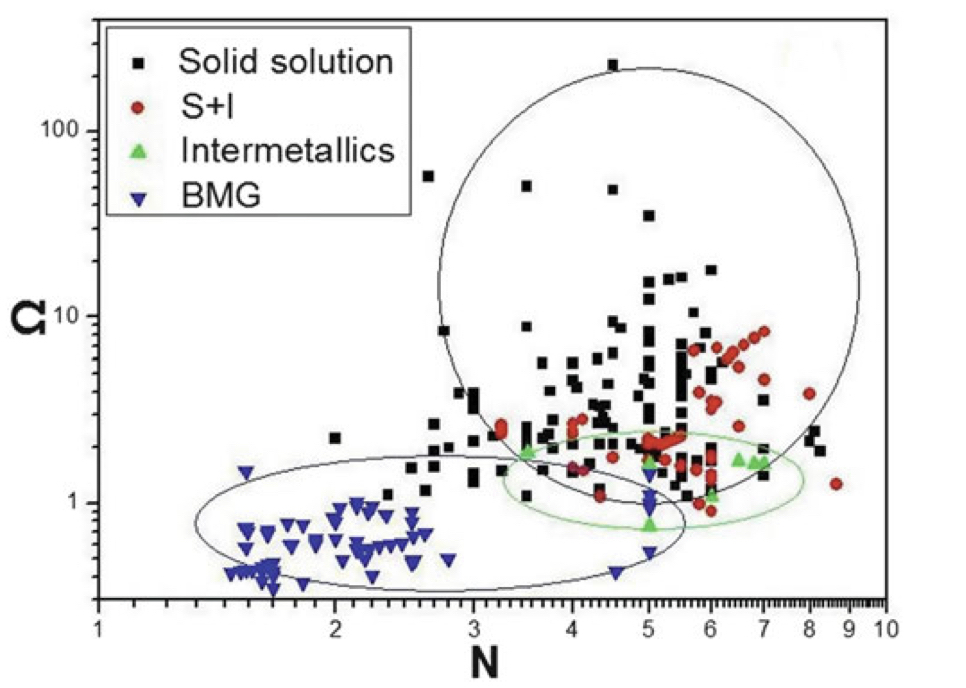
\includegraphics[width=\textwidth]{theory/heaformation1.jpeg}
\caption{HEA formation based on $\Omega$ and $\delta$}
\end{subfigure}
\begin{subfigure}{0.7\textwidth}
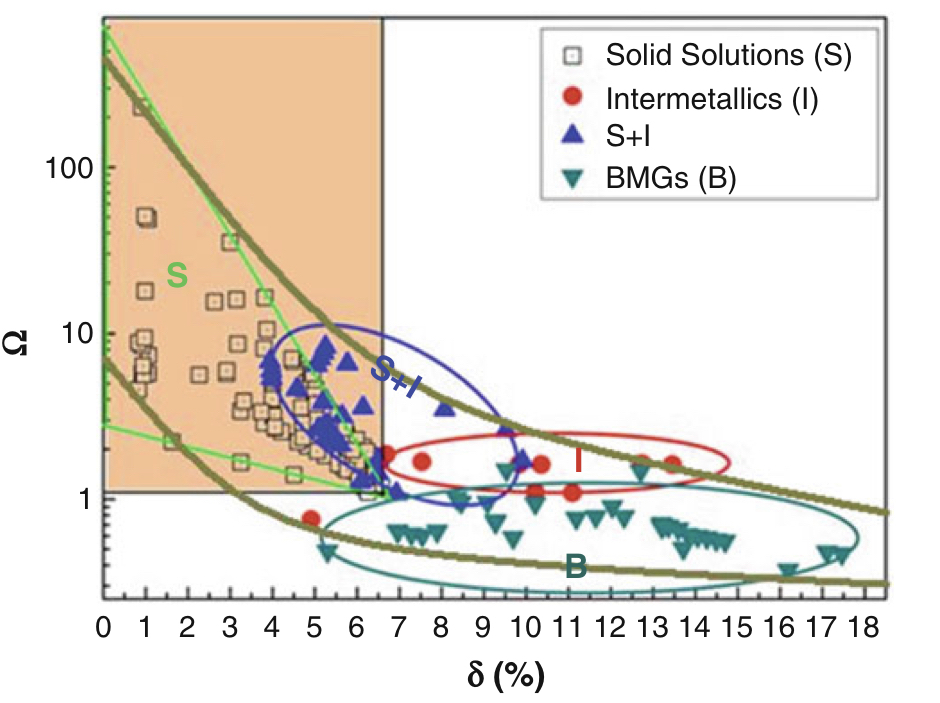
\includegraphics[width=\textwidth]{theory/heaformation2.jpeg}
\caption{HEA formation based on $\Omega$ and $N$}
\end{subfigure}
\caption{Formation of HEA based on $\delta$ and $N$. Figures adopted from \cite{hea2016_ch2}}
\label{Omega} 
\end{figure} 

An important quantity in terms of characterizing high-entropy alloys is the total number of electrons VEC. The valence electron concentration of a material is strongly related to the crystal structure of the material. For example, $Co_3V$, originally a hexagonal structure can be transformed into a tetragonal or cubic structure by either increasing the VEC from alloying with Ni, or reduction with Fe respectfully. Derived from the work of Guo et al. on the phase stability of a $Al_xCrCuFeNi_2$ HEA, the VEC can be directly related to the crystal structure of high-entropy alloys. A lower VEC stabilize the BCC phase, while higher values stabilize FCC. In between is a mixture of the two. Specifically values greater than 8.0 stabilize FCC, and values bellow 6.87 favor BCC. However, these boundaries is not rigid when including elements outside of transition metals, exceptions has also been found for high-entropy alloys containing $Mn$. All though a heavy majority of reported high-entropy alloys that form solid solutions have been found to adopt simple cubic structures such as FCC and BCC. Recent studies have observed HEA's in orthorombic structures like $Ti_{35}Zr_{27.5}Hf_{27.5}Ta_5Nb_5$ and hcp structures, for example $CoFeNiTi$.

\section{Core effects and properties}
Next, we will summarize the discussion above into four core elements that distinctly describe high-entropy alloys and their implications on the functional properties. The first of these is the "high-entropy effect", as the name suggests this is related to the increased configurational entropy from the amount of elements, that can inhibit the formation of strongly ordered structures. The second effect is the "severe lattice distortion effect", that originates from the fact that every element in a high-entropy structure is surrounded by non-homogeneous elements, thus leading to severe lattice strain and stress. The overall lattice distortion is additionally attributed to the differences in atomic size, bonding energies and crystal structure tendencies between the components. Therefore the total lattice distortion observed in HEA's are significantly greater than that of conventional alloys. This effect mostly affect the strength and conductivity of the material, such that a higher degree of distortion yields greater strength and greatly reduces the electronic and thermal conductivity due to increased electron and phonon scattering. An upside to this is that the scattering and following properties become less temperature dependent given that it originates from the lattice rather than thermal vibrations.
 
The two remaining effects, "sluggish diffusion" and "cocktail effect" can be summarized swiftly. The first is a direct consequence of the multi-component layout of high-entropy alloys that result in slowed diffusion and phase transformation because of the number of different elements that is demanded in the process. The most notable product from this effect is an increased creep resistance. Lastly we have the cocktail effect, which is identical to the smoothie analogy mentioned previously, in that the resultant characteristics is a combination of both the elements and their interaction. This is possible the most promising concept behind high-entropy alloys, which fuels researchers with ambition to discover highly optimized materials by meticulously combining and predicting properties from different elements. Examples of this can be the refractory HEA's developed by "Air Force Research Laboratory" severely exceeding the melting points and strength of previous Ni or Co-based superalloys by alloying specifically refractory elements such as Mo. Nb and W. Another example is the research conducted by Zhang et al. on the high-entropy system $FeCoNi(AlSi_{0-0.8}$ in the intent of unveiling the optimal combination of magnetic, electric and mechanical properties, resulting in an excellent soft magnet. 
\begin{figure} 
\centering
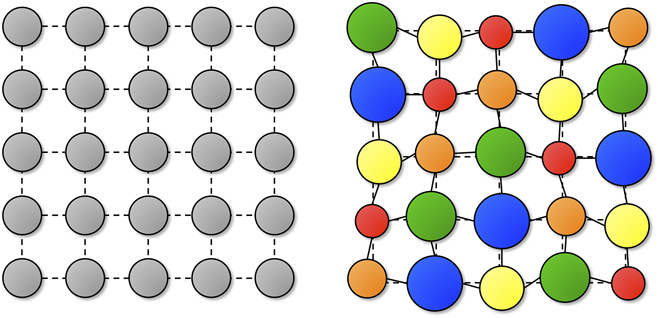
\includegraphics[width=\textwidth]{theory/latticeDistortionHEA.jpeg}
\caption{A schematic illustration of lattice distortion in high-entropy alloys. Figure from \cite{owen_jones_2018}}
\end{figure}

In the discussion above, we have covered the four core effects that make up high-entropy alloys and their relation to the mechanical and functional properties. Of the core effects, especially the lattice distortion and cocktail effect relate to the functional properties. Next we will include some examples from recent studies on the functional properties of HEAs.  


The initial study on the functional properties on high-entropy alloys was conducted on the H-x alloy, referring to the system $Al_xCoCrFeNi$ with $0 \leq x \leq 2$. It was found that the electrical resistivity was higher than that of conventional alloys, and that the conductivity generally decreased with increasing amounts of Al, additionally noteworthy low carrier mobility. Similar findings have also been made for the high-entropy alloy $FeCoNi(AlSi)_x$. 

\textbf{Write a small part on magnetic and relate to the cocktail effect, then very briefly conclude by mentioning findings of superconductivity, corrosion resistance, hydrogen storage and other properties/applications.}